
\subsection{Question 2.1.2}
La procédure d'initialisation des agents a été expliquée dans la partie précédente. 
Les paramètres suivants ont été affichés sur l'interface afin de pouvoir les modifier manuellement : Nc(nombre de consommateurs par groupe), nombres de fournisseurs par types, rounds-number(durée de la simulation), H(taille de la liste des notes par agent), initT (Valeur initiale de la température qui détermine la probabilité de choisir une action entre explorer et exploiter (dilemme de Boltzmann\cite{Dilemme}).

\begin{figure}[H]
\begin{center}
\begin{tabular}{|l|l|l|l|l|l|l|l|}
  \hline
  Nc & NPB & NPO & NPG & NPI & rounds-number & H & initT\\
  \hline
  500 & 45 & 40 & 10 & 5 & 500 & 10 & 1 \\
  \hline
\end{tabular}
\end{center}
\caption{Paramètres d'IT}
\end{figure}

Voici l'évolution des simulations jusqu'à l'obtention d'une figure similaire à la figure 9.
\begin{figure}[H]
   \begin{minipage}{0.48\textwidth}
     \centering
     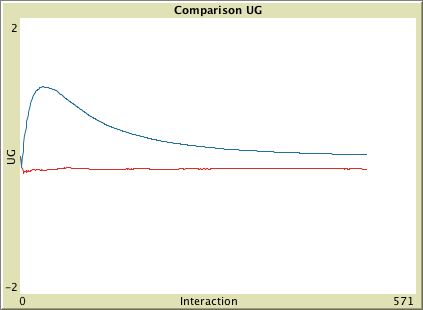
\includegraphics[width=.7\linewidth]{images/evolutionIT/IT1.png}
     \caption{IT-NoTrust : Plot 1}\label{Fig:Data1}
   \end{minipage}\hfill
   \begin{minipage}{0.48\textwidth}
     \centering
     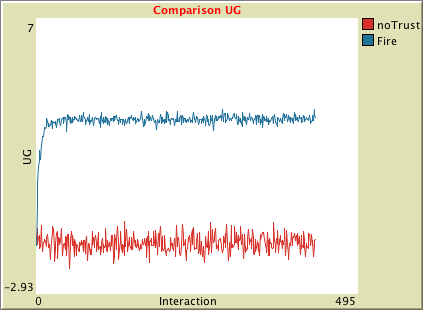
\includegraphics[width=.7\linewidth]{images/evolutionIT/IT2.png}
     \caption{IT-NoTrust : Plot 2}\label{Fig:Data2}
   \end{minipage}
\end{figure}

Le plot 1 représente la toute première courbe obtenue après l'implémentation des algorithmes. Nous pensions d'abord que la baisse après une trentaine d'itérations était dû à un H trop petit (taille de mémoire insuffisante). Finalement, nous avons obtenu le plot 2 après avoir inclus la prise en compte de la distance lors du calcul de $ER_{a2}$ (résultat attendu pour explore\cite{Dilemme}). En effet, la moyenne des niveaux de performances de tous les fournisseurs était retournée mais la distance à laquelle se trouvaient ces derniers n'était pas incluse dans le calcul. Il faut préciser, ici, que nous avions supposé (à tort) qu'un agent consommateur prenait la liste de tous les fournisseurs du monde avant sa sélection. A ce stade du projet (partie IT seule), nous n'avions pas remarqué qu'il ne prenait que ses voisins. Il arrivait donc que l'UG obtenue après une interaction soit très éloignée du $ER_{a2}$. Ceci a corrigé l'erreur du plot 1. 
\begin{figure}[H]
   \begin{minipage}{0.48\textwidth}
     \centering
     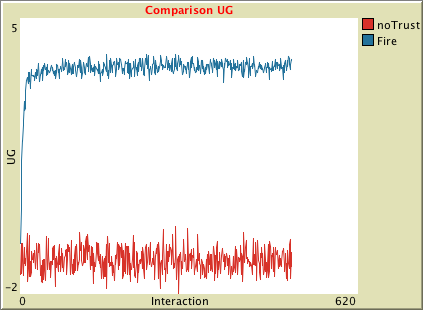
\includegraphics[width=.7\linewidth]{images/evolutionIT/IT3.png}
     \caption{IT-NoTrust : Plot 3}\label{Fig:Data1}
   \end{minipage}\hfill
   \begin{minipage}{0.48\textwidth}
     \centering
     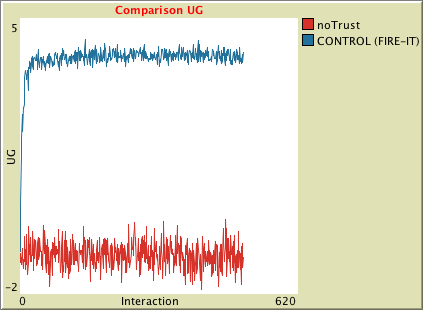
\includegraphics[width=.7\linewidth]{images/evolutionIT/IT4.png}
     \caption{IT-NoTrust : Plot 4}\label{Fig:Data2}
   \end{minipage}
\end{figure}

Ensuite, nous avons réussi à faire augmenter la moyenne en modifiant la variable T (température). Nous l'avons finalement initialisé à 1 puis diminué de 0.1\% à chaque interaction de l'agent.